% This file was created with tikzplotlib v0.10.1.
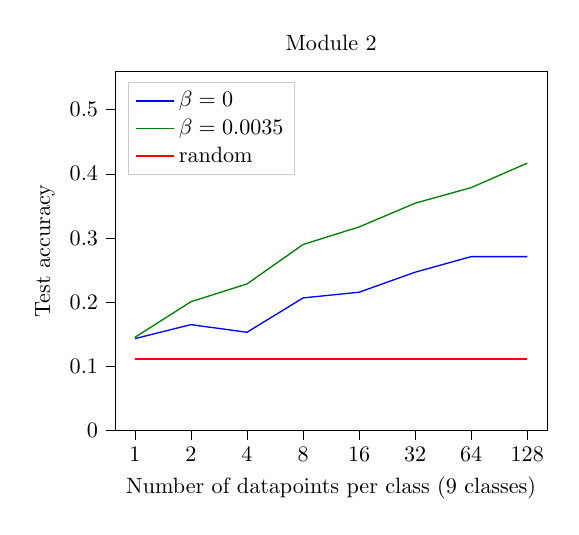
\begin{tikzpicture}[scale=0.8]

\definecolor{darkgray176}{RGB}{176,176,176}
\definecolor{green01270}{RGB}{0,127,0}
\definecolor{lightgray204}{RGB}{204,204,204}

\begin{axis}[
legend cell align={left},
legend style={
  fill opacity=0.8,
  draw opacity=1,
  text opacity=1,
  at={(0.03,0.97)},
  anchor=north west,
  draw=lightgray204
},
log basis x={2},
tick align=outside,
tick pos=left,
title={Module 2},
x grid style={darkgray176},
xlabel={Number of datapoints per class (9 classes)},
xmin=0.784584097896751, xmax=163.143760296865,
xmode=log,
xticklabels={0, 1,2,4,8,16, 32,64,128}, % <-- Modify xtick labels here
xtick style={color=black},
y grid style={darkgray176},
ylabel={Test accuracy},
ymin=0.0, ymax=0.559548593309191,
%ymin=0.0958333346048991, ymax=0.431944417741564,
ytick style={color=black}
]
\addplot [semithick, blue]
table {%
1 0.142857137407575
2 0.164682532719203
4 0.152777771949768
8 0.206349198477609
16 0.215277767181396
32 0.246527767181396
64 0.270833320617676
128 0.270833320617676
};
\addlegendentry{$\beta = 0$}
\addplot [semithick, green01270]
table {%
1 0.144841264316014
2 0.200396817071097
4 0.228174593108041
8 0.289682527269636
16 0.317129611968994
32 0.354166641235352
64 0.378472213745117
128 0.416666641235352
};
\addlegendentry{$\beta=0.0035$}
\addplot [semithick, red]
table {%
1 0.111111111111111
2 0.111111111111111
4 0.111111111111111
8 0.111111111111111
16 0.111111111111111
32 0.111111111111111
64 0.111111111111111
128 0.111111111111111
};
\addlegendentry{random}
\end{axis}

\end{tikzpicture}
